
% This LaTeX was auto-generated from MATLAB code.
% To make changes, update the MATLAB code and republish this document.

\documentclass{article}
\usepackage{graphicx}
\usepackage{color}

\sloppy
\definecolor{lightgray}{gray}{0.5}
\setlength{\parindent}{0pt}

\begin{document}

    
    

\section*{23. Nonlinear approximation: why rational functions?}

\begin{verbatim}
ATAPformats
\end{verbatim}
\begin{par}
Up to now, this book has been about polynomials, or in the last chapter, their transplants. The final six chapters of the book are about rational functions, which have been a mainstay of approximation theory from the beginning. Why do rational approximations occupy such a large place in the literature? Polynomials are familiar and comfortable, but rational functions seem complex and specialized. Is their position in approximation theory justified, or is it an artifact of history, perhaps a holdover from the pre-computer era? In this chapter we attempt to answer these questions, and in doing so we shall find ourselves considering the broader question of what the uses are of the whole subject of approximation theory.
\end{par} \vspace{1em}
\begin{par}
I think the answer is this.  Although rational functions indeed became an established part of approximation theory long before computers and many of today's practical applications, their place in the subject is deserved. Their importance stems from a conjunction of two facts.  On the one hand, rational functions are more powerful than polynomials at approximating functions \textit{near singularities} and on \textit{unbounded domains.} On the other hand, for various reasons related for example to partial fraction decompositions, they are easier to work with than their nonlinearity might suggest---indeed, sometimes no more complicated than polynomials.
\end{par} \vspace{1em}
\begin{par}
A rational function is the ratio of two polynomials, and in particular, given $m\ge 0$ and $n\ge 0$, we say that $r$ is a rational function of \textit{type} $(m,n)$ if it can be written as a quotient $p_m/q_n$ with $p_m\in {\cal P}_m$ and $q_n\in {\cal P}_n$.  The set of all rational functions of type $(m,n)$ is denoted by ${\cal R}_{mn}$, and any $r\in {\cal R}_{mn}$ can be written in the form $$ r(x) = \sum_{k=0}^m a_k x^k\kern -4pt \left/ \sum_{k=0}^n b_k x^k\right. \eqno (23.1) $$ for some real or complex coefficients $\{a_k\}$ and $\{b_k\}$.  The degrees need not be exact, i.e., there is no requirement that $a_m^{}$ or $b_n^{}$ must be nonzero. Nor do we require that the numerator and denominator are relatively prime, that is, that they have no common zeros.
\end{par} \vspace{1em}
\begin{par}
Suppose, however, that for some nonzero $r\in {\cal R}_{mn}$, we choose a representation with relatively prime numerator and denominator. Define $\mu \le m$ to be the index of the highest degree nonzero numerator coefficient and similarly $\nu\le n$ for the denominator, and further normalize the coefficients by requiring $b_\nu = 1$. Then we can write $$ r(x) = \sum_{k=0}^\mu a_k x^k\kern -4pt \left/ \sum_{k=0}^\nu b_k x^k \right. , \quad a_\mu\ne 0, ~b_\nu=1. \eqno (23.2) $$ In this case $r$ has exactly $\mu$ finite zeros and $\nu$ finite poles, counted with multiplicity: we say that $r$ is of \textit{exact type} $(\kern 1pt \mu,\nu)$. (The case in which $r$ is identically zero is a special one, with no nonzero coefficients in the numerator, and we say it has exact type $(-\infty,0)$.) If $\mu>\nu$, then $r$ has a pole at $x=\infty$ of order $\mu-\nu$, and if $\nu>\mu$ it has a zero at $x=\infty$ of order $\nu-\mu$.  Basic properties of rational functions are described in books of complex analysis such as [Ahlfors 1953, Henrici 1974, Markushevich 1985].
\end{par} \vspace{1em}
\begin{par}
These representations highlight the nonlinearity of rational functions, but a different perspective is suggested when we represent them by \textit{partial fractions.}  (Partial fractions were the subject of Jacobi's PhD thesis [1825], and an excellent general reference is Chapter 7 of [Henrici 1974].) In the simplest situation, consider $$ r(x) = \sum_{k=1}^n {c_k\over x-\xi_k}, \eqno (23.3) $$ where $\{\xi_k\}$ are distinct real or complex numbers. For any coefficients $\{c_k\}$, this is a rational function of type $(n-1,n)$. The number $c_k$ is the \textit{residue} of $r$ at $\xi_k$. This representation highlights the linear aspects of rational functions. For example, whereas computing the integral of $r$ written in the form $p/q$ looks daunting, in the representation (23.3) we have simply $$ \int^x r(s)ds = C + \sum_{k=1}^n c_k\log (x-\xi_k). \eqno (23.4) $$ In applications, it is interesting how often a formula like this turns out to be instrumental in making a rational function useful.
\end{par} \vspace{1em}
\begin{par}
The partial fraction form (23.3) does not apply to all rational functions.  One limitation is that it always represents a rational function of exact type $(\mu,\nu)$ with $\mu< \nu$. Another is that it does not represent all functions of this kind, since it cannot account for poles of multiplicity greater than $1$. The following theorem gives a partial fraction representation for the general case.
\end{par} \vspace{1em}
\begin{par}

{\bf Theorem 23.1.  Partial fraction representation.}
{\em Given $m,n\ge 0$, let $r\in {\cal R}_{mn}$ be arbitrary.  Then $r$ has
a unique representation in the form
$$ r(x) = p_0(x) + \sum_{k=1}^\mu p_k((x-\xi_k)^{-1}), \eqno (23.5) $$
where $p_0$ is a polynomial of exact degree $\nu_0$ for some
$\nu_0\le m$ {\rm (}unless $p=0)$ and $\{p_k\}$, $1\le k \le \mu$, are polynomials of exact
degrees $\nu_k\ge 1$ with $p_k(0)=0$ and}
$\sum_{k=1}^\mu \nu_k \le n$.

\end{par} \vspace{1em}
\begin{par}
\textit{Proof.} See Theorem 4.4h of [Henrici 1974]. $~\hbox{\vrule width 2.5pt depth 2.5 pt height 3.5 pt}$
\end{par} \vspace{1em}
\begin{par}
The function $p_0$ is the \textit{polynomial part} of $r$, and $p_k((x-\xi_k)^{-1})$ is its \textit{principal part} at $\xi_k$.
\end{par} \vspace{1em}
\begin{par}
This is all we shall say for the moment about the mathematics of rational functions. Let us now turn to the main subject of this chapter, the discussion of why these functions are useful in approximation theory and approximation practice.
\end{par} \vspace{1em}
\begin{par}
The right place to start is with a cautionary observation. Rational functions are not always better than polynomials. Indeed, consider the most basic of all situations, in which a fuction $f$ is analytic in a $\rho$-ellipse $E_\rho$ for some $\rho> 1$. For such a function, by Theorem 8.2, polynomial approximations will converge at the rate $O(\kern 1pt\rho^{-n})$.  It turns out that a typical convergence rate for type $(n,n)$ rational functions is $O(\kern 1pt\rho^{-2n})$.  So, doubling the number of parameters to be determined sometimes just approximately doubles the convergence rate. (In fact, sometimes it does not increase the convergence rate at all [Szabados 1970].) For applications of this kind, rational functions may outperform polynomials, but often it is by a rather modest factor.
\end{par} \vspace{1em}
\begin{par}
For example, here are a pair of curves showing $\|f-p_{2n}^*\|$ (dots) and $\|f-r_{nn}^*\|$ (stars) as functions of $n$ for $f(x) = \exp(-x^4)$, where $p_{2n}^*$ and $r_{nn}^*$ are the best approximations to $f$ in ${\cal P}_{2n}$ and ${\cal R}_{nn}$, respectively. (We shall discuss rational best approximation in the next chapter.) Both curves decrease geometrically, and there is not much difference between them.  (The rational approximations here should in principle be computed with \texttt{remez}, but Chebfun's rational remez algorithm is currently not robust enough, so \texttt{cf} is used instead.)
\end{par} \vspace{1em}
\begin{par}
 \vskip -2em 
\end{par} \vspace{1em}
\begin{verbatim}
x = chebfun('x'); f = exp(-x.^4); warning off
nn = 0:20; errp = []; errr = [];
for n = nn
  p2n = remez(f,2*n); errp = [errp norm(f-p2n,inf)];
  [p,q,foo] = cf(f,n,n); rnn = p./q; errr = [errr norm(f-rnn,inf)];
end
clf, semilogy(nn,errp,'.-','markersize',12), grid on, ylim([1e-16 10])
hold on, semilogy(nn,errr,'h-r','markersize',4), FS = 'fontsize';
text(10.5,2e-8,'E_{2n,0}',FS,10,'color','b')
text(9,1e-11,'E_{n,n}',FS,10,'color','r'), xlabel n
title(['Convergence of polynomial and rational '...
       'best approxs to exp(-x^4) on [-1,1]'],FS,9)
\end{verbatim}

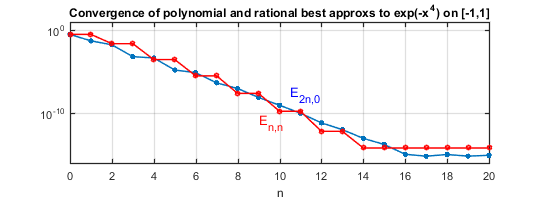
\includegraphics [width=4in]{chap23_01.png}
\begin{par}
 \vskip 1pt 
\end{par} \vspace{1em}
\begin{par}
What makes rational functions important is that, in contrast to this example, there are many problems where one wants to operate near singularities, or on unbounded domains.  For these problems, rational approximations may converge much faster than polynomials. For example, here is an experiment like the last one, but with $f(x) = |x|$. For this function, a type $(n,n)$ rational approximant with $n=150$ gives 16-digit accuracy, whereas polynomial approximants would need $n=10^{15}$ to do so well.  (Again this code should in principle use \texttt{remez} but cannot, so known best approximation errors are hardwired into the code.)
\end{par} \vspace{1em}
\begin{par}
 \vskip -2em 
\end{par} \vspace{1em}
\begin{verbatim}
f = abs(x); xx = linspace(-1,1,1000); nn = 0:50; errp = [];
errr = [.5 4.37e-2 8.50e-3 2.28e-3 7.37e-4 2.69e-4 1.07e-4 ...
        4.60e-5 2.09e-5 9.89e-6 4.88e-6 2.49e-6 1.30e-6 ...
        6.3*exp(-pi*sqrt(26:2:max(nn)))];
errr = kron(errr,[1 1]); errr(end) = [];
for n = nn
  p2n = remez(f,2*n); errp = [errp norm(f(xx)-p2n(xx),inf)];
end
hold off, semilogy(nn,errp,'.-','markersize',12), grid on
hold on, semilogy(nn,errr,'h-r','markersize',4)
text(37,3e-4,'E_{2n,0}',FS,10,'color','b')
text(21,2e-7,'E_{n,n}',FS,10,'color','r'), xlabel n
title(['Convergence of polynomial and rational '...
       'best approxs to |x| on [-1,1]'],FS,9)
\end{verbatim}

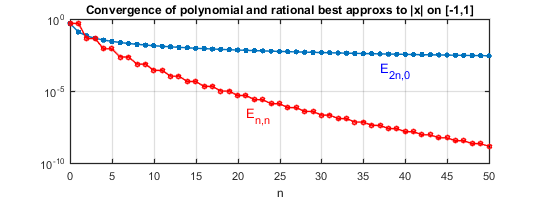
\includegraphics [width=4in]{chap23_02.png}
\begin{par}
 \vskip 1pt 
\end{par} \vspace{1em}
\begin{par}
The approximation of $|x|$ by rational functions is one of the ``two famous problems'' to be considered in Chapter 25.  Half a century ago Donald Newman proved that whereas polynomial approximants to $|x|$ converge just at the rate $O(n^{-1})$, for rational approximants the rate is $\exp(-C \sqrt n\kern 1pt)$ with $C>1$ [Newman 1964]. This result rigorously established the possibility of an exponential difference in effectiveness of the two types of approximations.
\end{par} \vspace{1em}
\begin{par}
The rest of this chapter is devoted to an outline of twelve applications in which rational approximations are useful.  In most of these examples, there is a singularity or unbounded domain in the picture. The exceptions are applications \#1 and \#8, where rational functions outperform polynomials less decisively.
\end{par} \vspace{1em}
\begin{par}
\textit{1. Elementary and special functions.} Classically, approximation theory brings to mind the problem of designing subroutines for computers to evaluate elementary functions, like $\sin(x)$, and special functions, like Airy or Bessel functions.   For some of these applications, especially when the number of digits of accuracy required is known in advance, rational approximations prove to be the best choice.  A classic project in this line is the SPECFUN software package [Cody 1993], descendant of the earlier FUNPACK [Cody 1975], which uses rational best approximations to evaluate Bessel functions, error functions, gamma functions and exponential integrals to 18 digits of accuracy. For many years a driving force behind these software products and an expert on the matter of practical rational approximations was W. J. Cody at the Argonne National Laboratory; Cody's version of the rational Remez algorithm is described in [Cody, Fraser \& Hart 1968]. For a presentation of some of the state of the art early in the 21st century, see [Muller 2006].
\end{par} \vspace{1em}
\begin{par}
\textit{2. Digital filters.}  In electrical engineering, the construction of low-pass, high-pass, and other digital filters often involves approximation of functions with jumps. (For these problems the approximation domain is usually the unit circle in the complex plane.) Jumps amount to singularities on or near the domain of approximation, and Theorem 8.3 implies that polynomials have no chance of rapid convergence for such functions. As Newman's theorem would lead us to expect, rational approximations sometimes do much better. Engineers use the term FIR (Finite Impulse Response) for polynomial filters and IIR (Infinite Impulse Response) in the rational case [Oppenheim, Schafer \& Buck 1999].
\end{par} \vspace{1em}
\begin{par}
\textit{3. Convergence acceleration for sequences and series.} The mathematical sciences are full of problems of extrapolation.  For example, one might be interested in $\lim_{h\to 0} f(h)$, where $f(h)$ is a quantity computed numerically on a grid of spacing $h$.  For such a problem, $f$ is often analytic at $h=0$, in which case \textit{Richardson extrapolation,} based on interpolating the data by a polynomial, may be beautifully effective. On the other hand, suppose we want to evaluate $\lim_{n\to \infty} a_n$ for a sequence $\{a_n\}$. We can regard this problem too as $\lim_{h\to 0} f(h)$ with the definition $f(1/n) = a_n$, but now, in many applications, $f(h)$ will not be analytic at $h=0$ and Richardson extrapolation will be ineffective.  The more powerful extrapolation methods that have been developed for such problems, such as Aitken extrapolation and the epsilon algorithm, are mostly based on rational approximations. See Chapter 28.
\end{par} \vspace{1em}
\begin{par}
\textit{4. Determination of poles.} Suppose a function $f$ is analytic on $[a,b]$ and has some real or complex poles nearby whose positions and residues are of interest. Classic examples of such problems arise in the study of phase transitions in condensed matter physics.  If we approximate $f$ by polynomials on $[a,b]$, then by Theorem 8.3, the convergence fails outside a $\rho$-ellipse of analyticity, so not much information about poles can be obtained. If we approximate by rational functions, exponential convergence to some of the poles can often be achieved. Specifically, a good strategy is to consider the poles of $r_{mn}$ for moderate values of $n$, where $r_{mn}$ is a rational approximant to $f$ obtained by $\hbox{Pad\'e}$ or $\hbox{Chebyshev--Pad\'e}$ approximation or rational interpolation or least-squares. See Chapters 26--28.
\end{par} \vspace{1em}
\begin{par}
\textit{5. Analytic continuation.} If $f$ is analytic on $[a,b]$, then in many applications it can be analytically continued, in theory, to the rest of the complex plane, apart from exceptional points and curves in the form of poles, other singularities, and branch cuts.  Computing such continuations numerically, however, is a difficult problem.  One could try approximating $f$ by a polynomial, but this approach will be useless outside the largest Bernstein ellipse in which $f$ is analytic. Rational functions, by contrast, may be effective for continuation much further out.  Again see Chapter 28.
\end{par} \vspace{1em}
\begin{par}
\textit{6. Eigenvalues and eigenvectors of matrices.} Suppose we want to compute an eigenvector of a matrix $A$. One approach, the \textit{power method,} is to pick a starting vector $x$ and compute $\lim_{n\to \infty}$ $A^n x$, but the convergence of this polynomial-based idea is very slow in general.  A much faster method, \textit{inverse iteration}, is based on rational approximations: find an approximation $\mu$ to some eigenvalue $\lambda$ and compute $\lim_{n\to\infty}$ $(A-\mu I\kern.7pt)^{-n} x$.  The convergence gets faster the closer $\mu$ is to the singularity $\lambda$, and exploitation of this effect leads to the spectacularly effective QR algorithm for matrix eigenvalues and eigenvectors [Francis 1961]. Experts in numerical linear algebra do not usually think about rational approximations when discussing inverse iteration or the QR algorithm, but such approximations come explicitly to the fore in the analysis of extensions such as shift-and-invert Arnoldi or rational Krylov iteration $\hbox{[G\"uttel}$ 2010].
\end{par} \vspace{1em}
\begin{par}
\textit{7. Model reduction and optimal control.} A major topic in numerical linear algebra and control theory is the approximation of complex input-output systems by simpler ones for more efficient computation. Via the Laplace transform, problems of this kind (in the case of continuous as opposed to discrete time) can in many cases be reduced to problems of approximation on the imaginary axis in the complex plane.  The unbounded domain makes rational approximations a natural choice, and in fortunate cases, a system with hundreds of thousands of degrees of freedom may be reduced to a model with just dozens or hundreds. One set of methods for such problems goes by the name of $H_\infty$ approximation, based on results by Adamyan, Arov and Krein [1971] and Glover [1984] that are related to CF approximation (Chapter 20). For more information see [Antoulas 2005, Zhou, Doyle \& Glover 1996, Embree \& Sorensen 2012].
\end{par} \vspace{1em}
\begin{par}
\textit{8. Exponential of a matrix.}  A famous paper in numerical analysis is ``Nineteen dubious ways to compute the exponential of a matrix'', by Moler and Van Loan in 1978, reprinted in expanded form 25 years later [Moler \& Van Loan 2003]. These authors compared many algorithms for computing $e^A$ and reached the conclusion that the most effective was a scaling-and-squaring method based on $\hbox{Pad\'e}$ approximation [Ward 1977].  Here, first $A$ is scaled so that its norm is on the order of $1$.  Then $e^A$ is approximated by $r(A)$, where $r$ is a type $(n,n)$ $\hbox{Pad\'e}$ approximant to $e^x$ (Chapter 27). This is an example where rational approximations outperform polynomials not decisively but by a more or less constant factor. This approach is used by the matrix exponential program \texttt{expm} in Matlab, which for many years was based on type $(6,6)$ $\hbox{Pad\'e}$ approximation. A more careful analysis of the scaling-and-squaring algorithm was later provided by Higham [2009], who concluded that a better choice was type $(13,13)$, and the \texttt{expm} code was adjusted accordingly in Matlab Version 8. In [Higham \& Al-Mohy 2010, Appendix] the authors conclude that $\hbox{Pad\'e}$ approximants are up to $23\%$ more efficient than Taylor polynomials in this application.
\end{par} \vspace{1em}
\begin{par}
\textit{9. Numerical solution of stiff PDEs.} A particularly important set of problems related to matrix exponentials are derived from partial differential equations.  The starting point of such applications is the Laplace operator $\Delta$ on a spatial domain $\Omega$ with Dirichlet boundary conditions, which has an infinite set of negative real eigenvalues diverging to $-\infty$. To solve the heat equation $\partial u/\partial t = \Delta u$ numerically on $\Omega$ with initial data $u(x,0) = u_0$, one would like to be able to compute the matrix exponential product $e^{tA} v_0$, where $A$ is a matrix discretization of $\Delta$ and $v_0$ is a discretization of $u_0$. The wide range of eigenvalues makes such a problem ``stiff'', posing challenges for numerical methods. One method for coping with stiffness is to find a rational function $r(x)$ that approximates $e^x$ accurately on $(-\infty,0\kern .5pt]$, hence in particular at all of the eigenvalues of $A$, and then to compute $r(tA)v_0$. Polynomials cannot approximate a bounded function on an infinite interval, but rational functions can. This problem of rational approximation of $e^x$ on $(-\infty,0\kern .5pt]$ goes back to Cody, Meinardus and Varga [1969], whose ``1/9 conjecture'', eventually settled by Gonchar and Rakhmanov [1986], is the other famous problem considered in Chapter 25. Generalizations have become important in scientific computing in recent years in the design of \textit{exponential integrators} for the fast numerical solution of stiff nonlinear ordinary and partial differential equations [Hochbruck \& Ostermann 2010, Kassam \& Trefethen 2005, Schmelzer \& Trefethen 2007].
\end{par} \vspace{1em}
\begin{par}
\textit{10. Quadrature formulas.} As we have seen in Chapter 19, a quadrature formula approximates an integral $I = \int_a^b f(x) dx$ by a finite linear combination $I_n = \sum_{k=0}^n w_k f(x_k)$. If the weights $w_k$ are interpreted as residues of a rational function $r(x)$ with poles at the nodes $x_k$, then by estimation of a Cauchy integral over a contour $\Gamma$ enclosing $[a,b]$ in the complex plane, one can show that the error $I-I_n$ is bounded in terms of the size of $f$ in the region enclosed by $\Gamma$ times the error in approximation of the analytic function $\log((x+1)/(x-1))$ by $r$ over the same region [Takahasi \& Mori 1971].  So every quadrature formula is connected with a rational approximation problem. In fact, Gauss's original derivation of the $(n+1)$-point Gauss quadrature formula on $[-1,1]$ was based on exactly this connection: he used type $(n,n+1)$ $\hbox{Pad\'e}$ approximation of $\log((x+1)/(x-1))$ at $x=\infty$ [Gauss 1814].
\end{par} \vspace{1em}
\begin{par}
\textit{11. Adaptive spectral methods for PDEs.} The barycentric interpolation formula has the form of a rational function that reduces to a polynomial for a special choice of weights (Chapter 5). Regardless of the choice of weights, however, one still gets an interpolant, and in some applications there is no compelling reason to force the interpolant to be a polynomial.  This opens up the possibility of much more flexible rational interpolants, which have the particular advantage of not being so sensitive to the distribution of the interpolation points. These ideas originated with Salzer [1981] and Schneider and Werner [1986], building on earlier work going as far back as Jacobi [1846], and were later developed by Berrut [1988], and Floater and Hormann [2007].  For ordinary and partial differential equations, they form the basis of adaptive spectral methods for solving problems whose solutions have singularities close to the region of approximation [Berrut, Baltensperger \& Mittelmann 2005, Tee \& Trefethen 2006, Hale \& Tee 2009].
\end{par} \vspace{1em}
\begin{par}
\textit{12. One-way wave equations.} Our final application became well known in the 1970s and 1980s [Halpern \& Trefethen 1988]. The usual wave equation permits energy propagation in all directions, but there are applications where one would like to restrict to half the permitted angles, a $180^\circ$ range.  For example, this idea is useful in underwater acoustics [Tappert 1977], in geophysical migration [Claerbout 1985], and in the design of absorbing boundary conditions for numerical simulations [Lindman 1975, Engquist \& Majda 1977]. How can we define a system that behaves like $u_{tt} = u_{xx} + u_{yy}$ for leftgoing waves, say, with negative $x$-component of velocity, while not propagating rightgoing waves?  (The subscripts represent partial derivatives.)  A Fourier transform shows that the dispersion relation of such a system should be $\xi = \omega \sqrt{1-s^2}$, where $s = \eta/\omega$ and $\omega, \xi, \eta$ are the dual variables to $t,x,y$.  Only the positive branch of the square root should be present, making this system a \textit{pseudodifferential operator.}  However, a rational approximation $\sqrt{1-s^2} \approx r(s)$ simplifies this to a differential equation. For example, the type $(2,2)$ $\hbox{Pad\'e}$ approximation $r(s) = (1-{3\over 4} s^2)/(1-{1\over 4} s^2)$ leads to the PDE $u_{xtt} - {1\over 4} u_{xyy} = u_{ttt} - {3\over 4} u_{tyy}$, sometimes known as the $\hbox{``}45^\circ$ equation'' because it has high accuracy approximately for angles up to $45^\circ$. In this application, rational functions are superior to polynomials both because of higher accuracy in view of the singularities at $s=\pm 1$, and because polynomial approximations lead to PDEs that are ill-posed [Trefethen \& Halpern 1986].
\end{par} \vspace{1em}
\begin{par}
We have just seen a list of twelve applications.  In concluding this chapter I would like to consider what light these may shed on the biggest question of all, namely, what is the use of approximation theory?
\end{par} \vspace{1em}
\begin{par}

To see some possible views, let us go back to 1901.  That was the year of
Runge's landmark paper (Chapter 13), whose title was\footnote{Title:
``\"Uber empirische Funktionen und die Interpolation zwischen
\"aquidistanten Ordinaten.''  First sentence: ``Die Abh\"angigkeit
zwischen zwei messbaren Gr\"ossen kann, strenge genommen, durch
Beobachtung \"uberhaupt nicht gefunden werden.''}

\end{par} \vspace{1em}
\begin{par}
 \em ``On empirical functions and interpolation between
equidistant ordinates.'' 
\end{par} \vspace{1em}
\begin{par}
In reading this today, one is struck by the word ``empirical''.  The empirical theme is echoed in the opening sentence:
\end{par} \vspace{1em}
\begin{par}

\em The relationship between two measurable quantities can, strictly
speaking, not be found by observation.

\end{par} \vspace{1em}
\begin{par}
Runge goes on to mention ``observations'' six times more in the opening paragraph.  It would seem that his motivation is the processing of scientific data: interpolation in the traditional sense of evaluating a function at points lying between those at which it is listed in a table.
\end{par} \vspace{1em}
\begin{par}

The next year, 1902, brought another landmark of approximation theory:
Kirchberger's PhD thesis under Hilbert in G\"ottingen, which included the
first systematic statement and proof of the equioscillation theorem for
polynomial approximation (Theorem 10.1). Here is the first paragraph of
Kirchberger's thesis, as reprinted in the first paragraph of his
published paper a year later [1903], setting forth a clear motivation for
approximation theory.  We may imagine that this was probably also
Hilbert's view of the subject.\footnote{``Mit dem Begriff der Funktion
ist das Postulat der numerischen Berechnung der Funktionswerte f\"ur
irgendwelche Werte der unabh\"angigen Variabeln gegeben.  Da aber die
vier elementaren Spezies der Addition, Subtraktion, Multiplikation und
Division, oder streng genommen nur die erste drei derselben, die einzigen
numerisch ausf\"uhrbaren Rechnungsarten, alle andern aber nur insoweit
durchf\"uhrbar sind, als sie sich auf diese zur\"uckf\"uhren lassen, so
folgt hieraus, dass wir s\"amtliche Funktionen nur insoweit numerisch
beherrschen, als sie sich durch rationale Funktionen ersetzen, d.~h.\
angen\"ahert darstellen lassen.  Hieraus erhellt die gro\ss e Bedeutung
der Ann\"aherungsprobleme f\"ur die gesamte Mathematik und die
ausgezeichnete Stellung, die die Probleme der Ann\"aherung durch
rationale oder ganze rationale Funktionen einnehmen.  In der Tat setzt,
wenigstens f\"ur die numerische Berechnung, jede Ann\"aherung durch
andere, z.~B. trigonometrische Funktionen, die ann\"aherungsweise
Ersetzbarkeit dieser Funktionen durch rationale voraus.''}

\end{par} \vspace{1em}
\begin{par}
 \em
The notion of a function entails the assumption that a numerical value of
the function can be calculated for any value of the independent variable.
But since the only operations that can really be carried out numerically
are the four elementary operations of addition, subtraction,
multiplication and division, or strictly speaking only the first three of
these, it follows that we are really only masters of more general
functions insofar as we can replace them by rational functions, that is,
represent them approximately. This highlights the great significance of
approximation problems for the whole of mathematics and the special role
of approximation by polynomials and rational functions.  Indeed, for
numerical calculation at least, any use of other approximations such as
trigonometric functions presupposes that these can in turn be
approximated by rational functions.

\end{par} \vspace{1em}
\begin{par}
Updated to 2012, we may say that Kirchberger's justification of approximation theory is all about \textit{machine arithmetic.} Approximation by polynomials and rational functions is important, he is saying, because ultimately computers can only carry out polynomial and rational operations.
\end{par} \vspace{1em}
\begin{par}
Both Runge's emphasis on data and Kirchberger's emphasis on arithmetic capture aspects of approximation theory that remain valid today.  In particular, Kirchberger's paragraph seems a remarkably clear statement of a justification of approximation theory that in a certain philosophical sense seems almost unarguable (although the line between ``primitive'' operations like $+$ and ``derived'' ones like $\sin(\cdot)$ is not always so clear on actual computers, with their multiple levels of hardware, software and microcode). The same argument is often seen nowadays.
\end{par} \vspace{1em}
\begin{par}
Nevertheless, I do not think data analysis or machine arithmetic get at the heart of why approximation theory is important and interesting.  In fact I don't think Runge's words even capture the truth of why \textit{he} was interested in the subject!  (He becomes more of a mathematician in the second half of his paper.) What these observations miss is the importance of \textit{algorithms.}
\end{par} \vspace{1em}
\begin{par}
Let us look again at the list of applications. Kirchberger's motivation could be said to be on target for \#1 and \#2 (evaluation of functions, digital filters), and Runge's for \#3, \#4, and \#5 (extrapolation, determination of poles, analytic continuation). But the remaining seven items need to be accounted for in other ways.  It is noteworthy that applications \#6 to \#9 all involve matrices, sometimes of very large dimension (eigenvalues and eigenvectors, model reduction, exponentials of matrices, stiff PDEs).  Applications \#9 to \#12 all involve integrals and differential equations (stiff PDEs, quadrature, adaptive spectral methods, one-way wave equations).  In most of these problems we seem a long way from scalars $x$ and $r(x)$: the polynomial and rational operations are applied to matrices and operators, not just numbers.
\end{par} \vspace{1em}
\begin{par}
Chebfun provides another interesting data point (for polynomials rather than rational functions).  Chebfun is built on a century of developments in polynomial interpolation and approximation, and it makes it possible to work with univariate functions numerically in almost unlimited ways. A particularly important Chebfun capability is finding roots of a function $f(x)$, which enables many further operations like computing extrema, absolute values, and 1-norms.  Chebfun finds the roots by the algorithm proposed by Good [1961] and Boyd [2002] and described in Chapter 18: approximate $f$ by polynomial interpolants, then find roots of the polynomials by computing eigenvalues of colleague matrices. This is as powerful an application of approximation theory as one could ask for, but it has little to do with data analysis or machine arithmetic.
\end{par} \vspace{1em}
\begin{par}

Why are polynomial and rational approximations useful? Not because
$r(x)$ is easier to evaluate than $\exp(x)$, but because $r(A)$ is easier
to evaluate than $\exp(A)$, and $r(\partial/\partial x)$ is easier to
evaluate than $\exp(\partial/\partial x)\kern .5pt$! Not because we can
{\em evaluate} $p(x)$, but because we can {\em find its roots\kern
1.5pt}!

\end{par} \vspace{1em}
\begin{par}

\begin{displaymath}
\framebox[4.7in][c]{\parbox{4.5in}{\vspace{2pt}\sl
{\sc Summary of Chapter 23.}
Rational functions are more powerful than polynomials for approximating
functions near singularities or on unbounded domains.  This is the
reason for their importance in approximation theory and approximation
practice.\vspace{2pt}}}
\end{displaymath}

\end{par} \vspace{1em}
\begin{par}
 \small\smallskip\parskip=2pt
\par
{\bf Exercise 23.1.  Examples of partial fractions.}
Express the following functions in partial
fraction form: (a) $x^3/(1-x)$ (b) $x/(x^2-4)$, (c) $x^2/(x^2-4)^2$,
(d) $(1-x^3) / (1+x^2)$.
\par
{\bf Exercise 23.2.  Uses of partial fractions.}
(a) Express the function $r(x) = (x(x+1)(x+2))^{-1}$ in
partial fraction form.  (b) What is its integral from $1$ to $t$?
(c) What is the sum of the infinite series $r(1) + r(2) + r(3) + \cdots\,$?
\par
{\bf Exercise 23.3.  Another infinite series.}
(a) Based on numerical experiments, conjecture a value of the
infinite sum $1/(1\cdot 3\cdot 5)
+ 2/(3\cdot 5\cdot 7)
+ 3/(5\cdot 7\cdot 9) + \cdots .$  (b) Verify your conjecture
with partial fractions.
\par
{\bf Exercise 23.4.  A trigonometric identity.}
Verify the identity $1/(1\cdot 3\cdot 5)
- 1/(7\cdot 9\cdot 11)
+ 1/(13\cdot 15\cdot 17) - \cdots  = \pi/48.$
\par
{\bf Exercise 23.5.  Polynomial vs.\ rational experiments.}  Produce
plots comparing $E_{2n,0}(f)$ and $E_{n,n}(f)$ for the following
functions $f$ defined on $[-1,1]:$ (a) $\log(1+x^2)$, (b)
$\tanh(5x)$, (c) $\exp(x)/(2-x)$.
\par
{\bf Exercise 23.6.  Approximation of a gamma function.}
Consider the function $f(x) = \Gamma(x+2)$ on $[-1,1]$, which has
simple poles at $x=-2, -3, \dots.$\ \ Determine analytically the
geometric convergence rates to be expected as $m\to\infty$ for rational
approximants to $f$ of types (a) $(m,0)$, (b) $(m,1)$, (c) $(m,2)$.
\par 
\end{par} \vspace{1em}



\end{document}
    
